
\begin{center}
\textbf{Préparation d'un échantillon de glace}
\end{center}

\textbf{ICE MEMORY} est un programme international qui vise à constituer des archives de la composition de l'air, pour analyser les évolutions et leur impact sur le climat.
Il s'agit de collecter des carottes de glace des glaciers à forte valeur scientifique parmi les plus exposés au changement climatique et de les stocker en Antarctique pour les scientifiques des générations futures.

\medskip

\emph{Source : www.cnrs.fr}

\medskip

Les analyses réalisées sur les carottes de glace permettent de mesurer les variations passées du climat, de l'environnement et, tout particulièrement, de la composition atmosphérique grâce aux micro-bulles piégées dans la glace : variations de la température, des concentrations atmosphériques des gaz à effet de serre, des émissions d'aérosols naturels ou de polluants d’origine humaine.

\medskip

\emph{Source : www.ice-memory.org}

\medskip

Afin d'effectuer des analyses de l'eau constituant la carotte, on fait fondre une tranche de carotte de glace de forme cylindrique de 1,0 cm d’épaisseur et 10 cm de diamètre
à l'aide d'un appareil de chauffage de puissance $P_0 = 500$ W. L'appareil atteint cette puissance en 15 secondes. On l'éteint à l'instant $t_f$ lorsque l'eau liquide obtenue par la fonte de la glace atteint $25 \degres$C.

La courbe représentée ci-après donne l'évolution de la puissance $P(t)$ fournie par l'appareil au cours du chauffage, avec $P(t)$ en W et $t$ en seconde.

Cette courbe est formée d'un segment de droite et d'une demi-droite parallèle à l'axe des abscisses.

\begin{center}
\begin{tikzpicture}
    % Axes
    \draw[->] (-0.3,0) -- (13,0) node[below] {$t$};
    \draw[->] (0,-0.3) -- (0,4) node[left] {$P(t)$};
    % Origine
    \node[below left] at (0,0) {0};
    % Graduations et labels
    \draw (0,3) -- (-0.1,3) node[left] {$500$};
    \draw (3,0) -- (3,-0.1) node[below] {$15$};
    \draw (11,0) -- (11,-0.1) node[below] {$t_f$};
    % Courbe
    \draw[line width=0.5mm] (0,0) -- (3,3) -- (11,3);
    % Hachures sous la courbe
    %\fill[pattern=north east lines, pattern color=red] (0,0) -- (3,3) -- (3,0) -- cycle;
    %\fill[pattern=north east lines, pattern color=blue] (3,3) -- (11,3) -- (11,0) -- (3,0) -- cycle;
\end{tikzpicture}

\medskip

\emph{Évolution de la puissance en fonction du temps au cours du chauffage avec $P(t)$ en W et $t$ en seconde.}
\end{center}

\subsection*{3.1.}
Hachurer sur le graphique précédent en respectant les légendes ci-dessous, le domaine dont l'aire vaut $\int_0^{15} P(t) \, dt$ et le domaine dont l'aire vaut $\int_{15}^{t_f} P(t) \, dt$. Préciser les valeurs de ces aires.

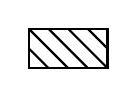
\begin{tikzpicture}
    % Clipper pour limiter les hachures à l'intérieur du rectangle
    \begin{scope}
        \clip (0,0) rectangle (1,0.5); % Définit la zone de découpe (rectangle)
        % Hachures inclinées
        \foreach \x in {-2,-1.75,...,6} {
            \draw[thick] (\x,0) -- (\x-0.5,0.5);}
    \end{scope}
    % Rectangle (bordure)
    \draw[thick] (0,0) rectangle (1,0.5);
\end{tikzpicture}
: aire correspondant à $\int_0^{15} P(t) \, dt$

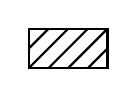
\begin{tikzpicture}
    % Clipper pour limiter les hachures à l'intérieur du rectangle
    \begin{scope}
        \clip (0,0) rectangle (1,0.5); % Définit la zone de découpe (rectangle)
        % Hachures inclinées (de bas à gauche vers haut à droite)
        \foreach \x in {-2,-1.75,...,6} {
            \draw[thick] (\x,0) -- (\x+0.5,0.5);}
    \end{scope}
    % Rectangle (bordure)
    \draw[thick] (0,0) rectangle (1,0.5);
\end{tikzpicture}
: aire correspondant à $\int_{15}^{t_f} P(t) \, dt$

\subsection*{3.2.}
Donner l'expression de $\int_0^{t_f} P(t) \, dt$ en fonction de $t_f$.

\subsection*{3.3.}
Donner l'expression de $P(t)$ pour $t$ appartenant à l'intervalle $[0 ; 15]$. Donner une primitive de $P$ sur l'intervalle $[0 ; 15]$. Retrouver la valeur de $\int_0^{15} P(t) \, dt$.

\subsection*{4.}
Déterminer l'instant $t_f$ en supposant que, pour faire fondre la glace et à porter l'eau liquide obtenue à $25 \degres$C :
\begin{itemize}
\item une énergie totale d’environ 37 kJ est nécessaire,
\item \textbf{toute l'énergie fournie par le chauffage est utilisée à cette tâche}.
\end{itemize}
On utilisera le résultat obtenu à la question \textbf{3.2}.

\subsection*{5.}
En réalité, le temps de chauffe est de 1 min 45 s. Commenter.

\bigskip


